\documentclass[8pt]{beamer}

\usepackage{verbatim}
\usepackage[english]{babel}
\usepackage[utf8]{inputenc}
\usepackage[T1]{fontenc}
\usepackage{csquotes}

\usepackage{expl3, biblatex}
\usepackage{algorithm2e, program}

\addbibresource{references.bib}

\usepackage{booktabs}
\usepackage{amsmath, bm}
\newcommand{\matrva}[1]{\bm{#1}} % recomended by ISO
\newcommand{\vecc}[1]{\bm{#1}} % recomended by ISO
\usetheme{Berlin}

\title{Latent diffusion models, stable diffusion, sdxl, and control nets}
\author{Justin Barry}
\date{\today}
% \subject{Presentation Subject}
% \keywords{the, presentation, keywords}
\begin{document}



\begin{frame}[plain]
\maketitle
\end{frame}



\begin{frame}{Intro}
    \textbf{Main idea}: Using diffusion models (DM) to generate an image given a text describing the image, dubbed "text-to-image". 
\end{frame}



\begin{frame}{Problem}
    Diffusion Models (DMs) for Image Synthesis
    \begin{itemize}
        \item DMs aim to learn an image distribution by gradually denoising a distribution of noisy images.
    \end{itemize}
\end{frame}



\begin{frame}{Novelties}
    Novel additions ~\cite{rombach2022highresolution}
    \begin{itemize}
        \item Conditioning on text via cross-attention mechanism.
        \item Performing denoising objective in a compressed latent space as opposed to the original pixel space.
        \item Model that transforms conditioning inputs and yields a representation for both images and texts.
        \item 1.45B parameters
    \end{itemize}
\end{frame}



\begin{frame}{To the point}
   \begin{figure}
       \centering
       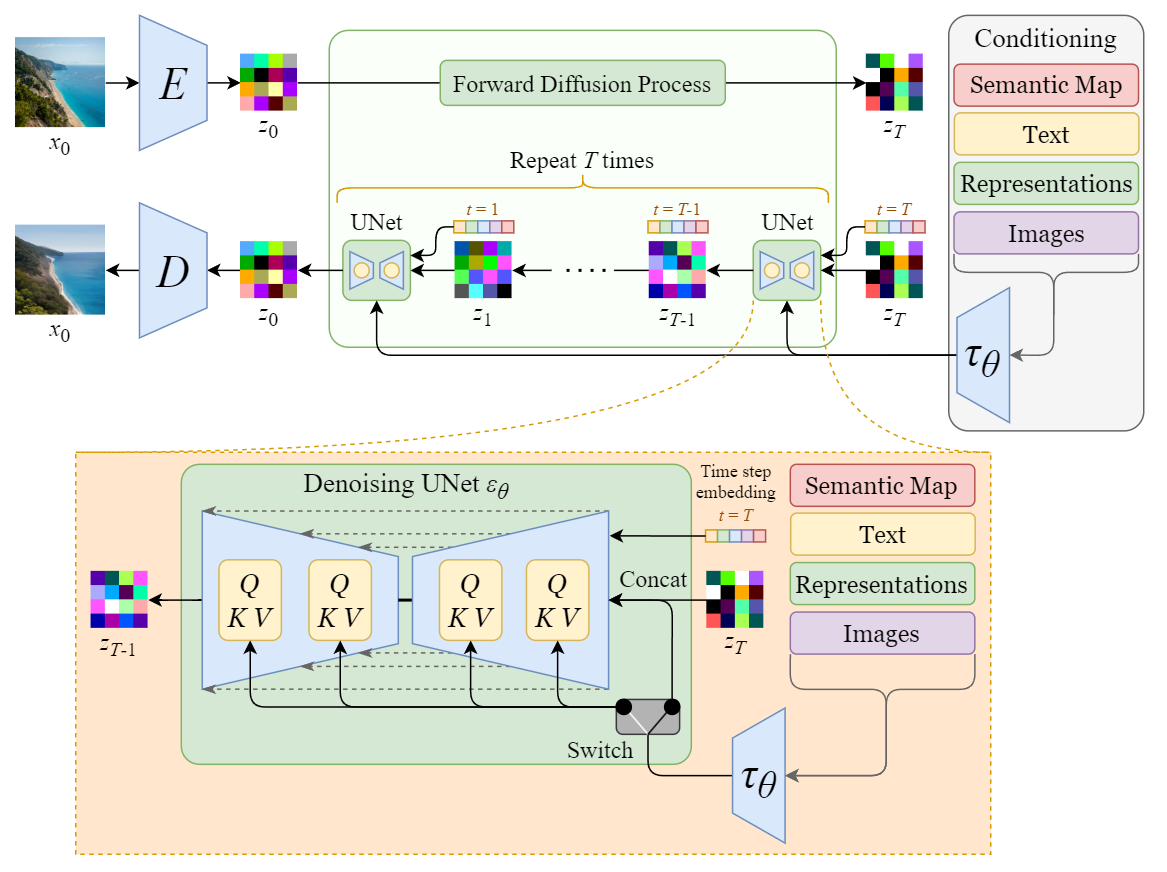
\includegraphics[width=276pt, height=165pt]{images/model.png}
       \label{fig:NN_training}
   \end{figure} 
   \cite{steins}
\end{frame}



\begin{frame}{Model annotated}
   \begin{figure}
       \centering
       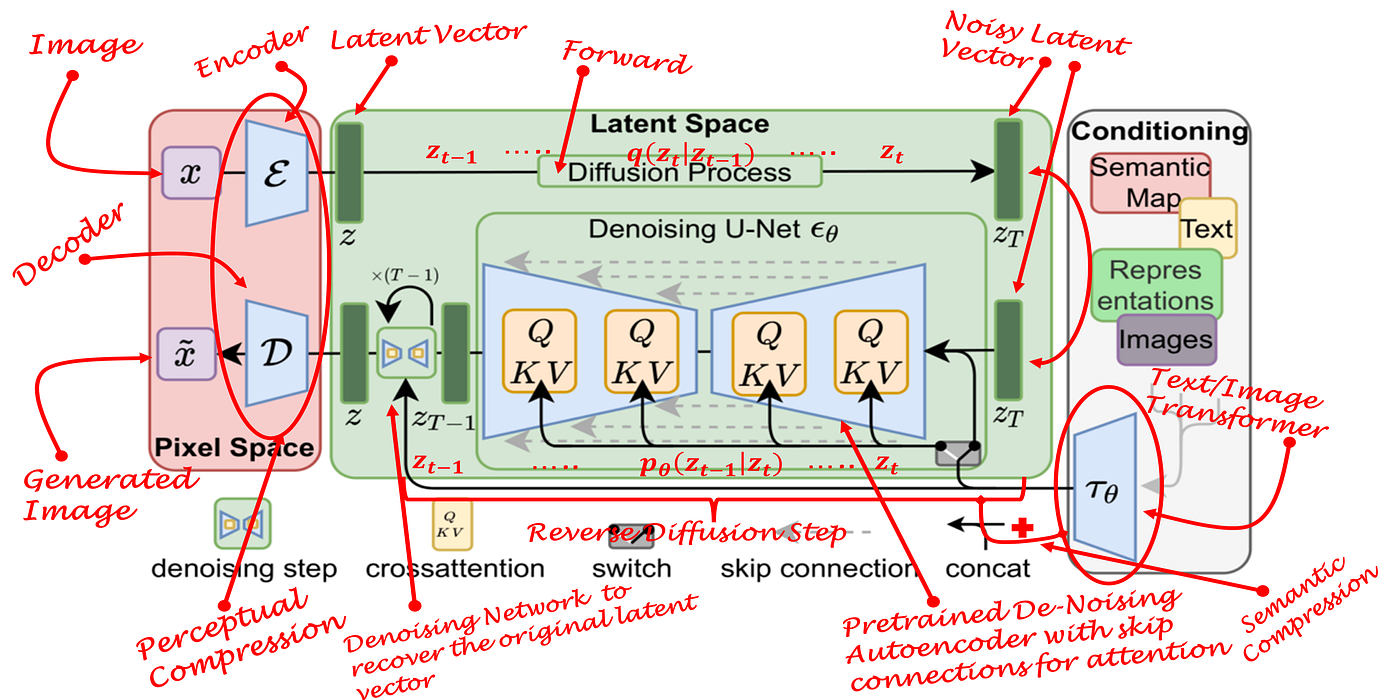
\includegraphics[width=276pt, height=165pt]{images/model_diagram_annotated.png}
       \label{fig:NN_training}
   \end{figure} 
   \cite{steins}
\end{frame}



\begin{frame}{Computational complexity}
    \begin{itemize}
        \item Problem: high complexity computing the diffusion model over the original images (pixel space).
        \item Solution: The authors' approach is to apply DMs in the latent space yielded by autoencoders.
        \item Two components to stable diffusion:
        \begin{itemize}
            \item The autoencoder compresses images to the latent space.
            \item U-net to denoise latent images (our diffusion model).
        \end{itemize}
    \end{itemize}
\end{frame}



\begin{frame}{Perceptual compression model}
    \begin{itemize}
        \item Avoid function evaluation in the pixel space by leveraging image compression.
        \item A reconstructed image
            \begin{align*}
                \Tilde{x} = \mathcal{D}(z) = \mathcal{D}(\mathcal{E}(x))
            \end{align*}
        \item $\mathcal{E}$ encoder
        \item $\mathcal{D}$ decoder
        \item $x$ original image
        \item $z$ latent (compressed) image
    \end{itemize}
   \begin{figure}
       \centering
       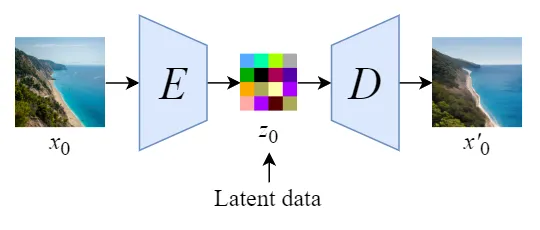
\includegraphics[width=150pt, height=75pt]{images/perceptual_loss_encoder.png}
       \label{fig:NN_training}
   \end{figure} 
   \cite{steins}
\end{frame}



\begin{frame}{Perceptual compression loss}
    Autoencoder objective
    \begin{align*}
        L_{autoencoder} &= \underset{\mathcal{E},\mathcal{D}}{min}\:\underset{\Psi}{max} (L_{rec}(x, \mathcal{D}(\mathcal{E}(x))) - L_{adv}(\mathcal{D}(\mathcal{E}(x))) + \log \mathcal{D}_{\Psi}(x) + L_{reg}(x;\mathcal{E}, \mathcal{D})) \\
        &= L_{reconstruction} + L_{adversarial} + L_{regularization}
    \end{align*}
    \begin{itemize}
        \item $L_{reconstruction}$ computes the loss over the feature space, not the pixel space
        \item $L_{adversarial}$ Is the total loss from an adversarial game between the autoencoder and a discriminator
        \item $L_{regularization}$ ensures the latent space and the predictive image distribution don't stray from a normal distribution.
    \end{itemize}
\end{frame}



\begin{frame}{Image generation}
    \begin{itemize}
        \item Diffusion: A function that adds noise images gradually.
        \item Problem: How to generate images.
        \item Solution: Learn the reverse diffusion process to generate images from noise.
    \end{itemize}
   \begin{figure}
       \centering
       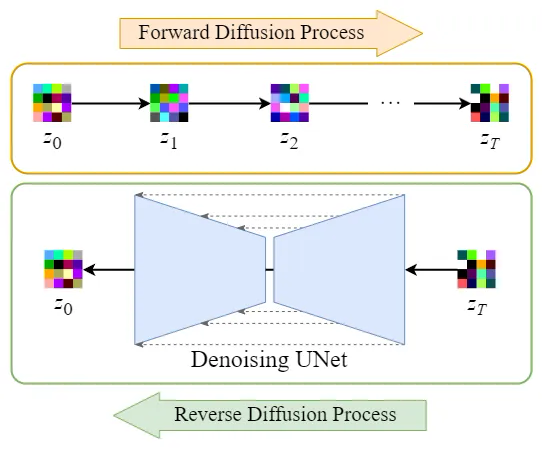
\includegraphics[width=200pt, height=150pt]{images/forward_backward_pass.png}
       \label{fig:NN_training}
   \end{figure} 
   \cite{steins}
\end{frame}


\begin{frame}{Abilities \& tasks}
    \begin{itemize}
        \item Text-to-image
        \begin{itemize}
            \item Class conditional image synthesis.
            \item Text prompt describing the image.
        \end{itemize}
        \item Image-to-image
        \begin{itemize}
            \item Semantic synthesis: condition on semantic map.
            \item Super resolution: condition on low-resolution image.
            \item Inpainting: condition on masked regions of the image.
        \end{itemize}
    \end{itemize}
\end{frame}



\begin{frame}{Notes on training and data}
    \begin{itemize}
        \item Training data contains images paired with a condition (image, text) or (image, image)
        \item LAION-400M language prompts.
        \item Finetuning on COCO.
        \item Evaluation data MS-COCO validation set.
        \item Classifier-free guidance greatly boosts sample quality.
    \end{itemize}
\end{frame}



\begin{frame}{Goal}
    \begin{itemize}
        \item We want a model that can generate a meaningful image from noise.
        \item A diffusion function describes how noise is gradually added to an image overtime.
        \item We can apply the diffusion function in reverse to generate meaningful images from noise.
        \item The authors leverage a mechanism to condition on text that guides image generation
    \end{itemize}
\end{frame}



\begin{frame}{Training objective}
    \begin{columns}
        \begin{column}{0.5\textwidth}
            \textbf{Unconditional training objective} learn a latent image distrubution $p(z)$ by gradually denoising the latent image. Find $\theta$ that minimizes the following
            \begin{align*}
                L_{LDM} = \mathbb{E}_{\mathcal{E}(x), \epsilon \sim \text{N}(0,1)} \lVert \epsilon - \epsilon_{\theta}(z_t, t) \rVert_2^2
            \end{align*}
            \begin{itemize}
                \item $\epsilon$ the added noise
                \item $\epsilon_{\theta}(z_t, t)$ The predicted noise added to the original image
                \item $z_t$ is the noised image
                \item t is a timestep embedding of the same dimensions as z that acts as contextual guidance denoising U-Net model
            \end{itemize}
        \end{column}
        \begin{column}{0.5\textwidth}
           \begin{figure}
               \centering
               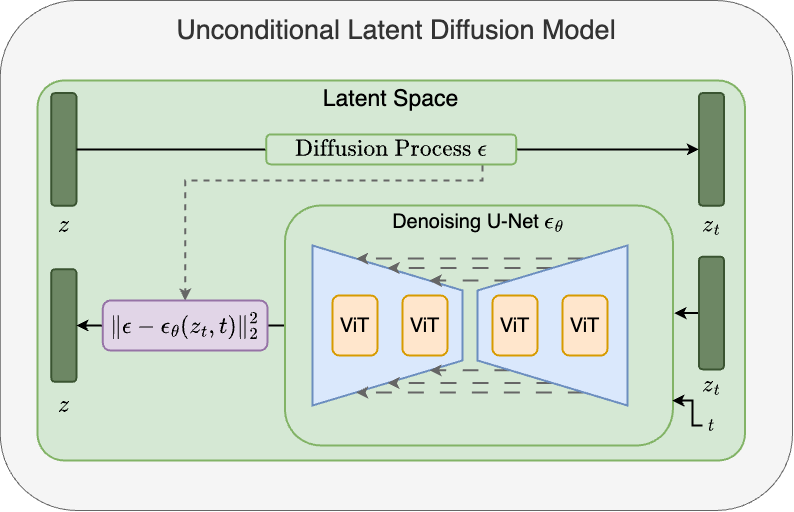
\includegraphics[scale=0.2]{images/sd_unconditional_objective}
               \label{fig:NN_training}
           \end{figure}
        \end{column}
    \end{columns}
\end{frame}



\begin{frame}{U-net}
    U-net is an autoencoder with skip connections from the encoders to the decoders that preserve the loss of spatial information during the encoding.
   \begin{figure}
       \centering
       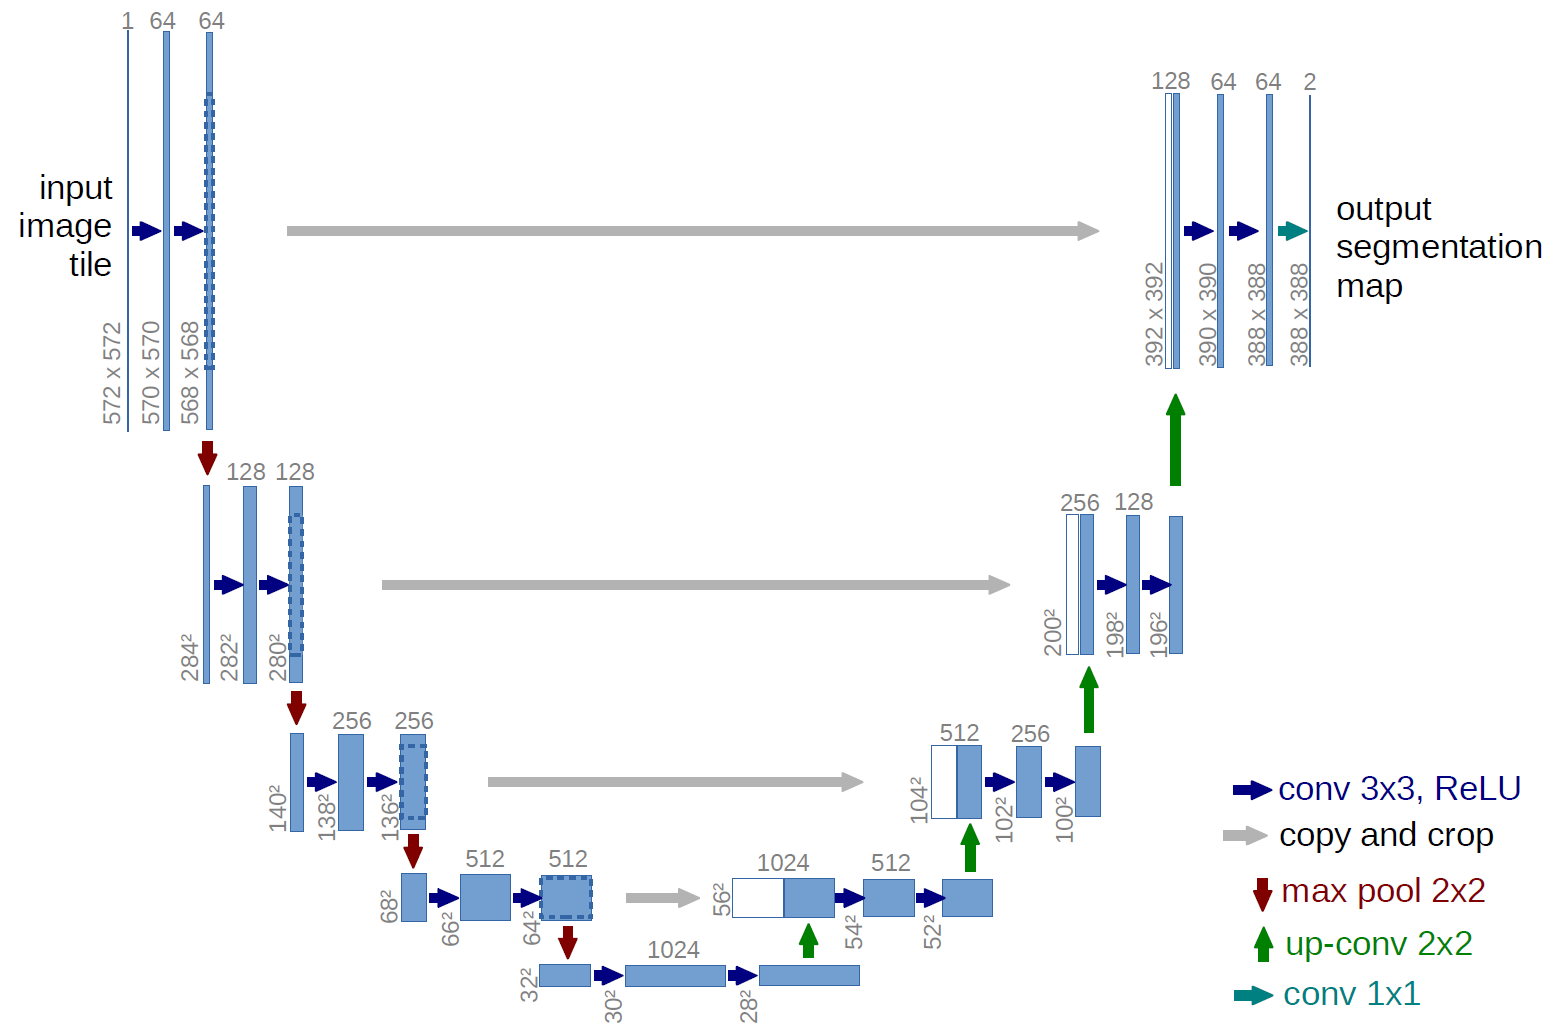
\includegraphics[scale=0.10]{images/u-net-architecture}
       \label{fig:NN_training}
   \end{figure}
   \cite{uni_unet}
\end{frame}



\begin{frame}{Diffusion function}
    The diffusion function $q(z_t \mid z_0) = N(z_t \mid \alpha_t z_0, \sigma_t^2I)$ determines the amount of noise we add to images.
    \begin{itemize}
        \item $z_0$ is the original latent image.
        \item $z_t$ is the noised latent image at timestep $t$.
        \item $\alpha_t$ is the scaling factor at timestep $t$.
        \item $\sigma^2_t$ represents the variance of the noise at timestep $t$.
        \item $N$ denotes a normal distribution.
        \item $I$ represents the identity matrix, indicating that the noise is isotropic
    \end{itemize}
\end{frame}



\begin{frame}{Diffusion function (continued)}
    Noise schedule
    \begin{itemize}
        \item Training iterations do NOT correspond to timesteps $t$
        \item Total number of timesteps $\lvert T \rvert$ and scaling factors $\alpha_t$ are preset hyperparamters.
        \item Each $t$ will have a corresponding scaling factor $\alpha$
        \item The noise "progression" is determined by randomly assigning $t$ values to images at the beginning of each training iteration.
    \end{itemize}
\end{frame}



\begin{frame}{Learning the diffusion function}
    \begin{columns}
        \begin{column}{0.5\textwidth}
            To learn the diffusion function
            (note about time step embeddings for learning reverse)
            \begin{itemize}
                \item At the beginning of each iteration, randomly assign a time step $t$ to latent image $z_0$
                \item Add noise to the compressed image according to the schedule: $z_t = \alpha_t z_0 + \sigma_t^2\epsilon$
                \item Predict the noise added to the latent image using our model $\epsilon_{\theta}(z_t, t)$
                \item Calculate and backpropagate the loss given by $\| \epsilon - \epsilon_{\theta}(z_t, t) \|$
            \end{itemize}
           \cite{steins}
        \end{column}
        \begin{column}{0.5\textwidth}
           \begin{figure}
               \centering
               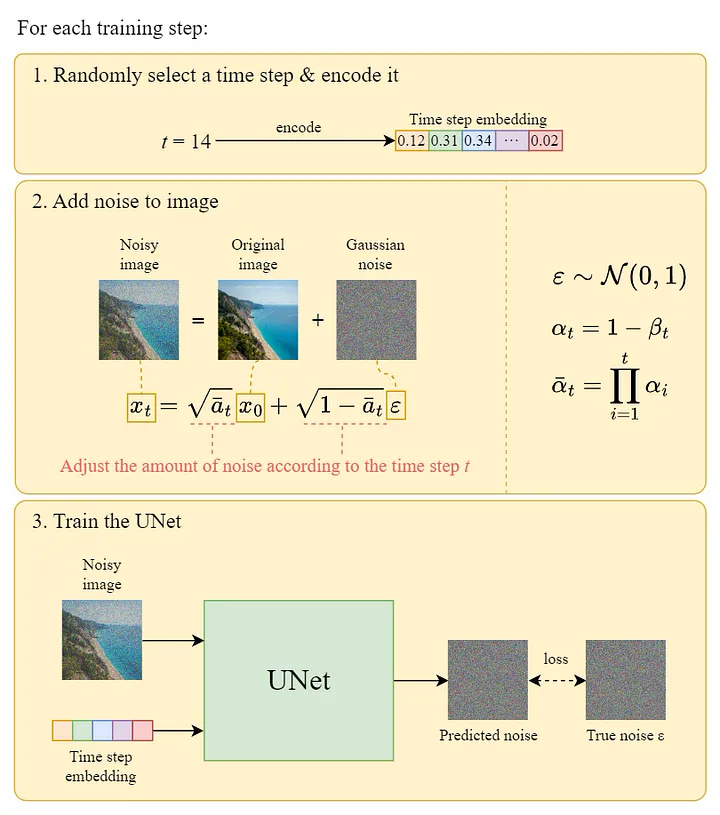
\includegraphics[width=150pt, height=150pt]{images/add_noise_via_schedule.png}
               \label{fig:NN_training}
           \end{figure}
        \end{column}
   \end{columns}
\end{frame}



\begin{frame}{Learning the diffusion function (continued)}
    \begin{columns}
        \begin{column}{0.5\textwidth}
            \begin{itemize}
                \item The model learns the diffusion function by randomly distributing the diffusion schedule across images.
                \item This is done by randomly assigning t's to z's (images).
                \item Computationally efficient: the model doesn't have to see each image at all stages of diffusion.
            \end{itemize}
        \end{column}
        \begin{column}{0.5\textwidth}
           \begin{figure}
               \vfill
               \hfill
               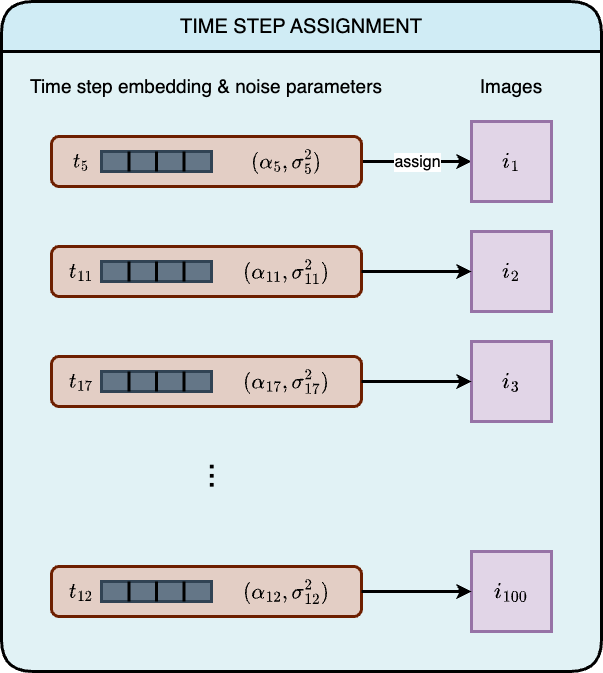
\includegraphics[width=130pt, height=130pt]{images/time_schedule_assignment.png}
               \label{fig:NN_training}
           \end{figure}
        \end{column}
   \end{columns}
\end{frame}



\begin{frame}{Conditioning the model}
    Stable diffusion can condition on both text and images.
    \begin{itemize}
        \item Conditional denoising autoencoder $\epsilon_{\theta}(z_t, t, y)$, where $y$ is our condition (text or image).
        \item Transform $y$ using CLIP to get an embedding: $\tau_{\theta}(y)$
        \item Reparameterize to get
        \begin{align*}
            L_{LDM} = \mathbb{E}_{\mathcal{E}(x), \epsilon \sim \text{N}(0,1)} \lVert \epsilon - \epsilon_{\theta}(z_t, t, \tau_{\theta}(y)) \rVert_2^2
        \end{align*}
    \end{itemize}
   \begin{figure}
       \centering
       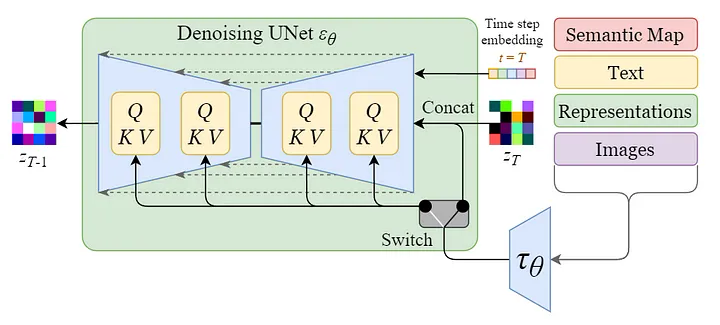
\includegraphics[scale=.35]{images/unet_text_condition.png}
       \label{fig:NN_training}
   \end{figure}~\cite{steins}
\end{frame}



\begin{frame}{Text transformer}
    \begin{itemize}
        \item SD leverages CLIP to implement $\tau_{\theta}$.
        \item CLIP uses a text encoder and an image encoder to learn a similarity score in a shared embeddings space.
    \end{itemize}
   \begin{figure}
       \centering
       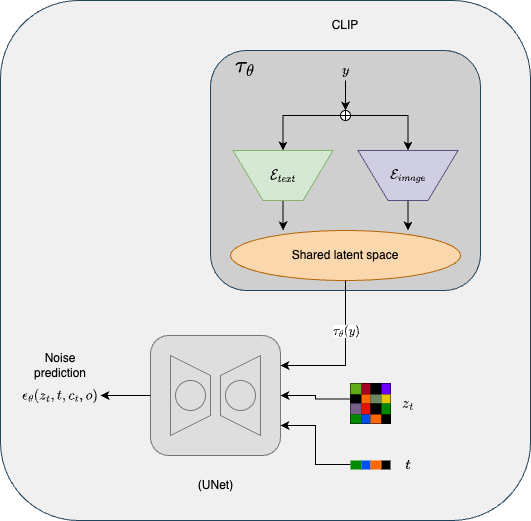
\includegraphics[scale=.27]{images/sd_with_clip}
       \label{fig:sd_with_clip}
   \end{figure}
\end{frame}



\begin{frame}{CLIP}
    How does CLIP work?
    \begin{itemize}
        \item CLIP maximizes the normalized dot product of images and their text descriptions (labels).
        \item The image and text encoders are both implemented by a transformer.
        \item Objective: maximize the the dot product between image and text embeddings.
    \end{itemize}
   \begin{figure}
       \centering
       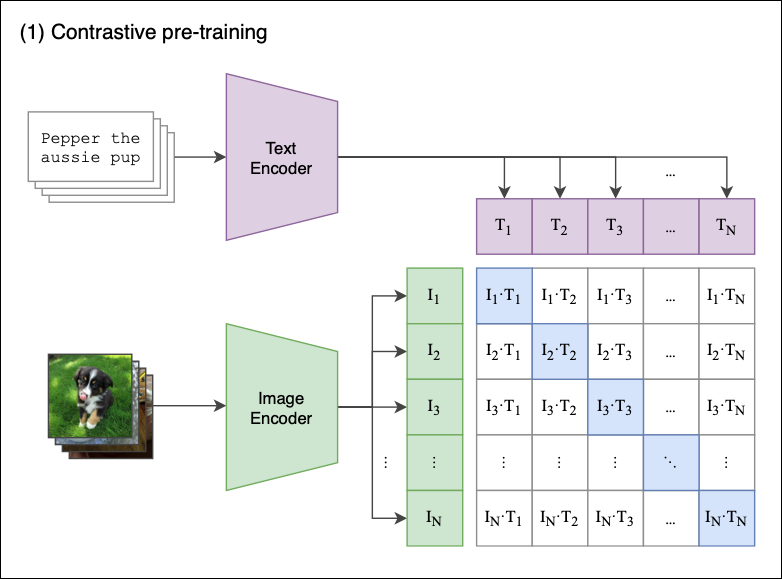
\includegraphics[scale=.16]{images/clip_model_architecture}
       \label{fig:unet_text_condition}
   \end{figure}~\cite{clip}
\end{frame}



\begin{frame}{CLIP in SD}
    \begin{itemize}
        \item $\tau_{\theta}(y)$ is a representation an image or text that is jointly learned in a shared embeddings space.
    \end{itemize}
\end{frame}



\begin{frame}{CLIP drawback}
    \begin{itemize}
        \item From AssemblyAI "In particular, many users of Stable Diffusion 2 have claimed that it cannot represent celebrities or artistic styles as well as Stable Diffusion 1, despite the fact that the training data for Stable Diffusion 2 was not deliberately filtered to remove artists. This discrepancy stems from the fact that CLIP's training data had more celebrities and artists than the LAION dataset. Since CLIP's dataset is not available to the public, it is not possible to recover this same functionality using the LAION dataset alone. In other words, many of the canonical prompting methods for Stable Diffusion 1 are all but obsolete for Stable Diffusion 2."~\cite{assamblyaiclip}
    \end{itemize}
\end{frame}



\begin{frame}{Cross attention in Stable Diffusion}
   \begin{itemize}
       \item The output of the text transformer $\tau_{\theta}(y)$ is passed to each block in U-net.
       \item $\tau_{\theta}(y)$ is the key $K$ in the cross attention operation for each block it's passed to.
   \end{itemize}

   \begin{columns}
      \begin{column}{0.5\textwidth}
         \begin{figure}
            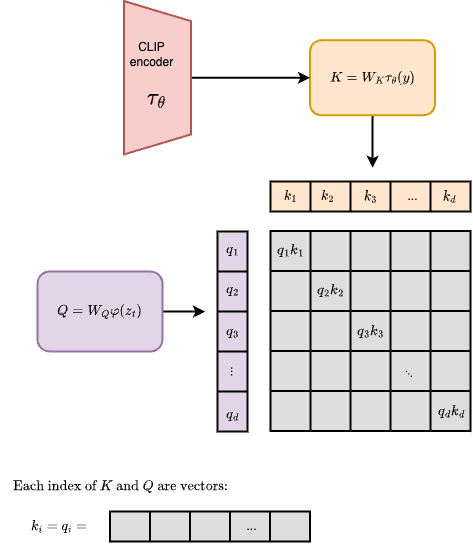
\includegraphics[scale=0.25]{images/sd_cross_attention_light}
            \label{fig:diffusion_process_diagram}
         \end{figure}
      \end{column}
      \begin{column}{0.5\textwidth}
        \begin{minipage}{\textwidth}
             \begin{figure}
                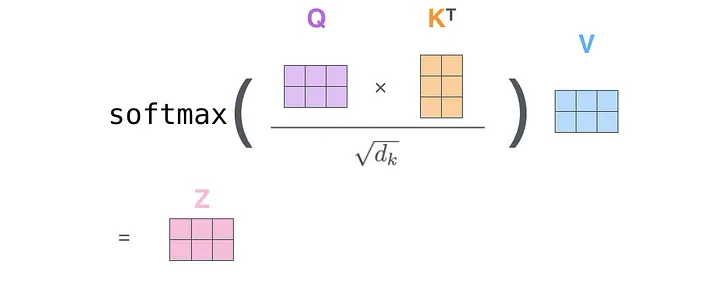
\includegraphics[scale=0.20]{images/qkv}
                \label{fig:image_generation_algorithm}
             \end{figure}
        \end{minipage}
        \begin{minipage}{\textwidth}
             \begin{figure}
                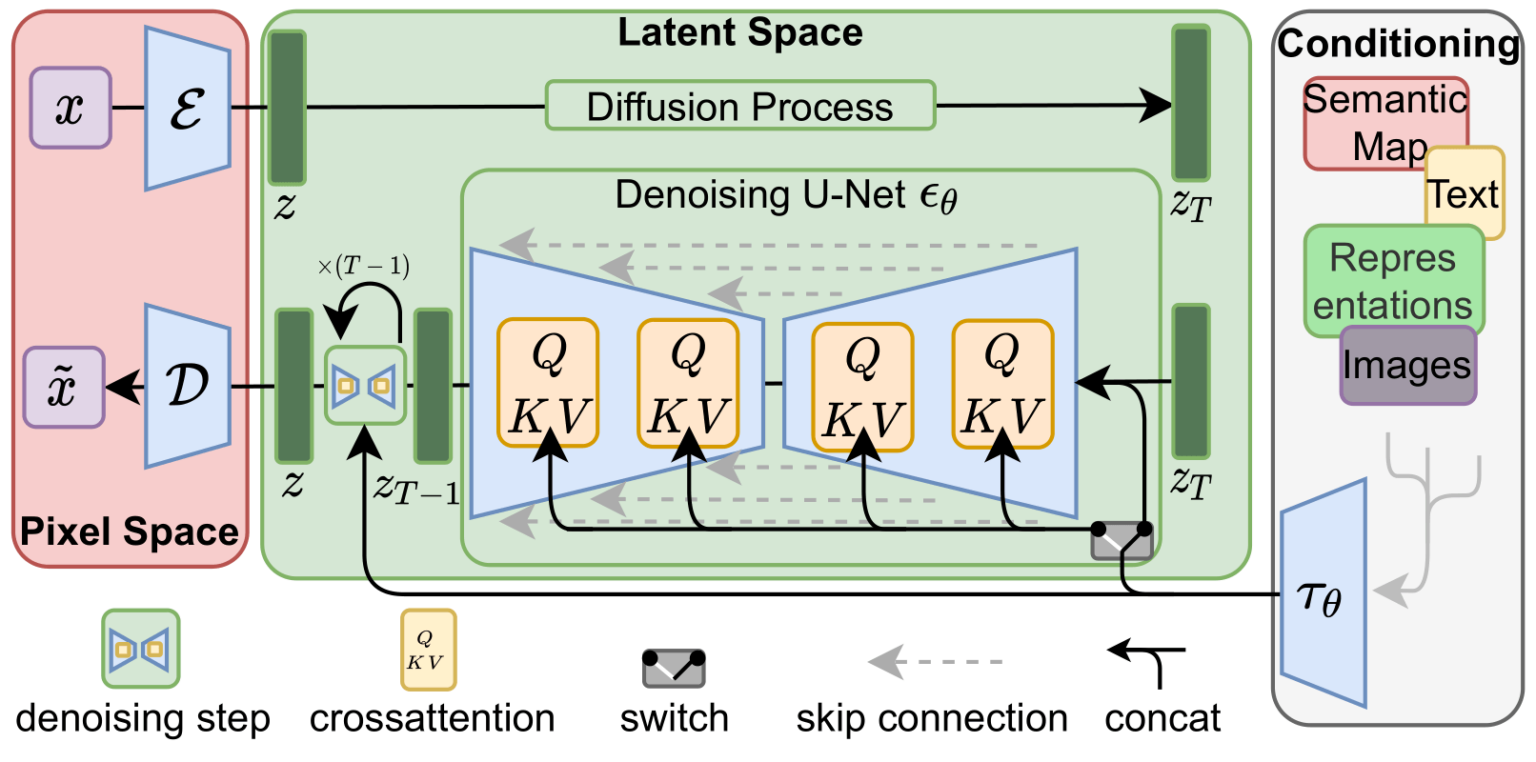
\includegraphics[scale=0.09]{images/sd_non_annotated}
                \label{fig:image_generation_algorithm}
             \end{figure}~\cite{rombach2022highresolution}
        \end{minipage}
      \end{column}
   \end{columns}
\end{frame}



\begin{frame}{Classifier-free guidance}
    \fontsize{7pt}{7pt}\selectfont
    \begin{columns}
        \begin{column}{.5\textwidth}
            Classifier-free guidance (CFG)~\cite{ho2022classifierfree} guides sd to place emphasis on inputs with prompts over inputs without prompts.
            \begin{align*}
                \epsilon_{final} &= \epsilon_{uc} + \beta(\epsilon_c - \epsilon_{uc}) \\
                &= \beta\epsilon_{c} + (1 - \beta)\epsilon_{uc}
            \end{align*}
            \begin{itemize}
                \item $\epsilon_c$ conditional image: has a prompt.
                \item $\epsilon_{uc}$ no prompt or masked prompt.
                \item A user defined weight $\beta$
                \item This effectively removes the influence of the unconditional image from the final prediction.
            \end{itemize}
        \end{column}
        \begin{column}{.5\textwidth}
           \begin{figure}
               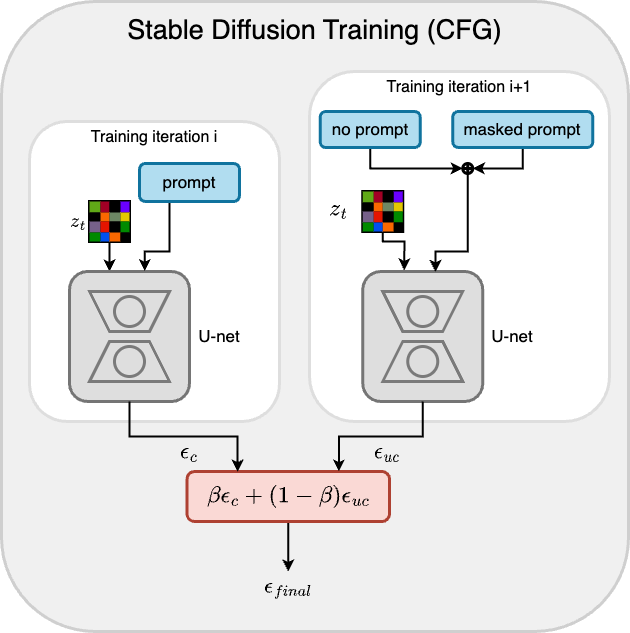
\includegraphics[scale=0.23]{images/sd_cfg}
               \label{fig:diffusion_process_diagram}
           \end{figure}
        % 627x633
        \end{column}
    \end{columns}
\end{frame}



\begin{frame}{CFG}
    The effect of the linear combination is the same as having two models, one for unconditional images and one for conditional images, each parameterized separately, but trained jointly
\end{frame}



\begin{frame}{Negative prompts}
    \fontsize{7pt}{7pt}\selectfont
    \begin{columns}
        \begin{column}{.5\textwidth}
            Negative prompts allow us to use prompts that describe what we DON'T want in an image to modify the output.
            \begin{itemize}
                \item Using the equation from~\cite{ho2022classifierfree} we get
                \begin{align*}
                    \epsilon_{final} = (1 + \beta)\epsilon_{c} - \beta \epsilon_{n}
                \end{align*}
                \item $\epsilon_{n}$ a negative prompt.
                \item This modifies the latent image by removing the aspects captured by the negative prompt.
            \end{itemize}
        \end{column}
        \begin{column}{.5\textwidth}
           \begin{figure}
               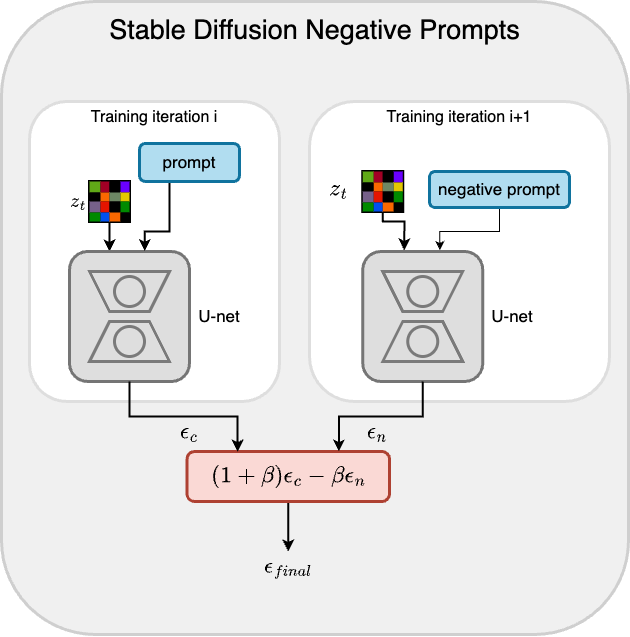
\includegraphics[scale=0.23]{images/sd_negative_prompts}
               \label{fig:sd_negative_prompts}
           \end{figure}
        % 627x633
        \end{column}
    \end{columns}
\end{frame}



\begin{frame}{Image generation}
   \begin{figure}
       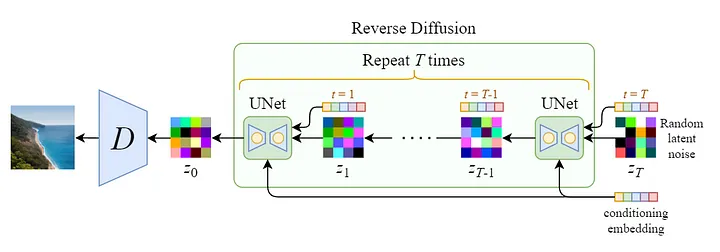
\includegraphics[scale=0.35]{images/diffusion_process_diagram}
       \label{fig:diffusion_process_diagram}
   \end{figure}
   \begin{figure}
       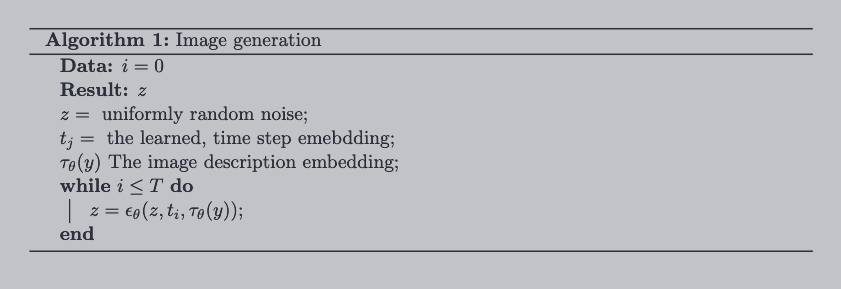
\includegraphics[scale=0.18]{images/image_generation_algorithm}
       \label{fig:image_generation_algorithm}
   \end{figure}
   \cite{steins}
\end{frame}



\begin{frame}{Stable Diffusion XL (SDXL)}
    \begin{columns}
        \begin{column}{.5\textwidth}
            \fontsize{6pt}{8pt}\selectfont
            SDXL~\cite{podell2023sdxl} improves SD to produce higher quality images
            \begin{itemize}
                \item Additions:
                \begin{itemize}
                    \fontsize{6pt}{8pt}\selectfont
                    \item A 3x larger unet-backbone.
                    \item Shift bulk of transformer computation to lower levels of U-net
                    \item Uses two text-image encoders (OpenCLIP ViT-bigG, CLIP ViT-L)
                    \item Additional text conditioning on pooled text embedding from OpenCLIP.
                    \item Conditioning (image size, aspect ratio, cropping coordinates)
                    \item Improved image compression variational autoencoder.
                    \item A refiner model to improve the visual quality of samples.
                    \item Uses openclip, a public model, instead of the private clip model from openai.
                \end{itemize}
            \end{itemize}
        \end{column}
        \begin{column}{.5\textwidth}
           \begin{figure}
               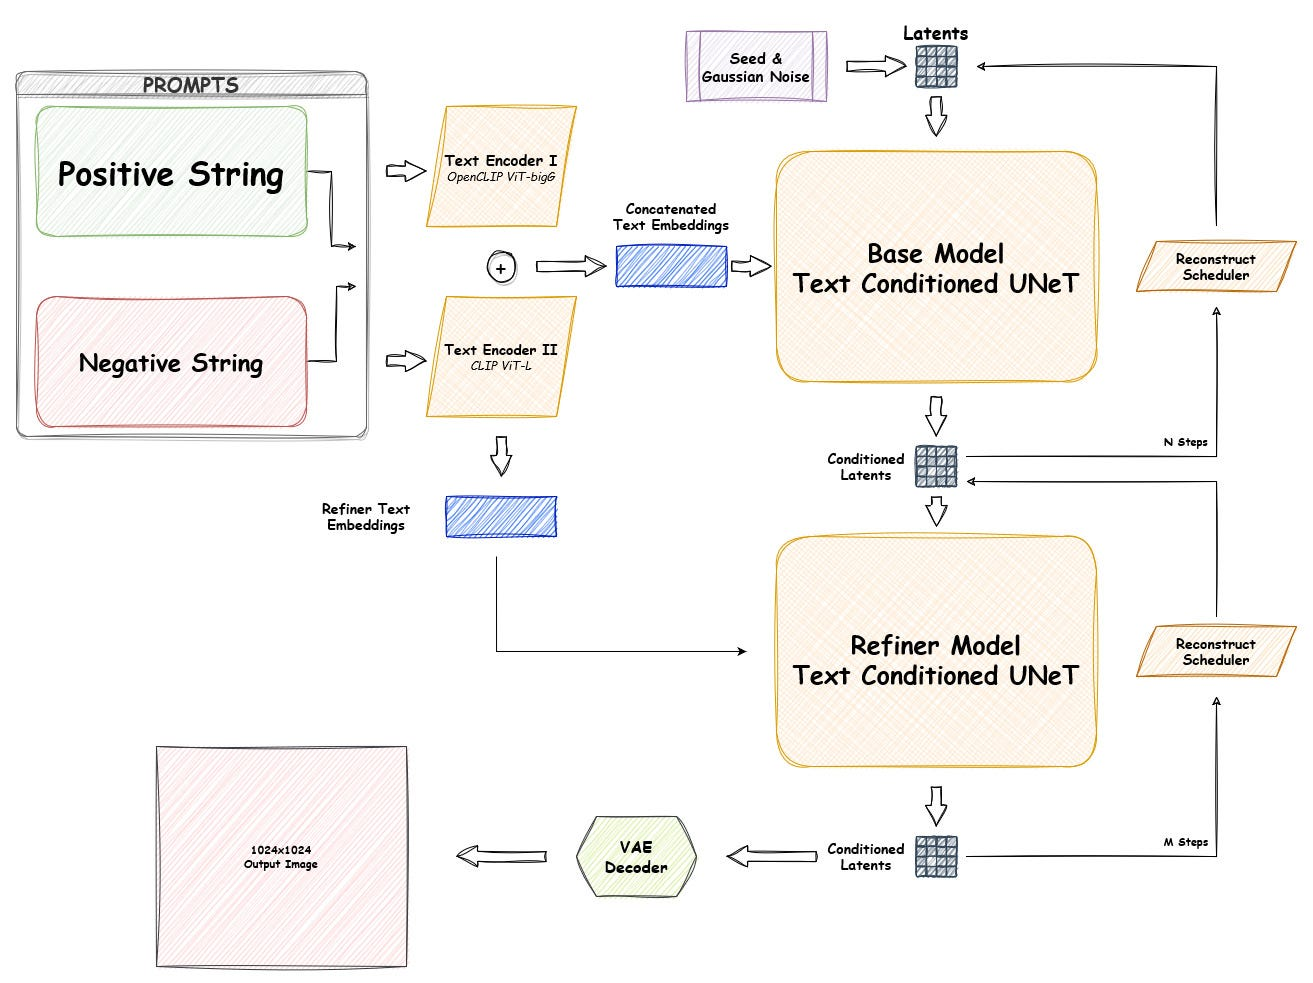
\includegraphics[scale=0.1]{images/sdxl_architecture}
               \label{fig:sdxl_architecture}
           \end{figure}~\cite{demir}
        \end{column}
    \end{columns}
\end{frame}



\begin{frame}{SD image size minimum}
    Loss of training data.
    \begin{itemize}
        \item The original SD model has a minimum threshold for image resolution.
        \item Trivial solution
        \begin{itemize}
            \item (1) Discard or (2) upscale image samples that below the threshold.
            \item (1) Leads to loss of \~39\% of data, degrading model performance.
            \item (2) Can introduce noise.
        \end{itemize}
    \end{itemize}
\end{frame}



\begin{frame}{Conditioning on image size}
    To solve for the problems introduced by the image size minimum, the author's condition SDXL on image size
    \begin{itemize}
        \item The original width and height of the image are added as conditioning features.
        \item Embed width and height individually using fourier feature encoding
        \item Concatenate embeddings and add to timestep embedding as input
    \end{itemize}
    \vspace{0.3cm}
    During inference, we can now change the generated image size based on the the conditioning paramters.
\end{frame}



\begin{frame}{Cropped objects in SD}
    \begin{columns}
        \begin{column}{0.5\textwidth}
            Problem: cropping leaking into generated images
            \begin{itemize}
                \item Different image sizes in a batch
                \item Crop images in a batch to match the target size
            \end{itemize}
            \vspace{0.3cm}
            solution
            \begin{itemize}
                \item Sample crop coordinates unfiormly at random.
                \item Transform the coordinates into Fourier feature embeddings.
                \item Concatenate the coordinate and size embeddings along the channel axis
                \item Feed as input to condition the model.
            \end{itemize}
        \end{column}
        \begin{column}{0.5\textwidth}
           \begin{figure}
               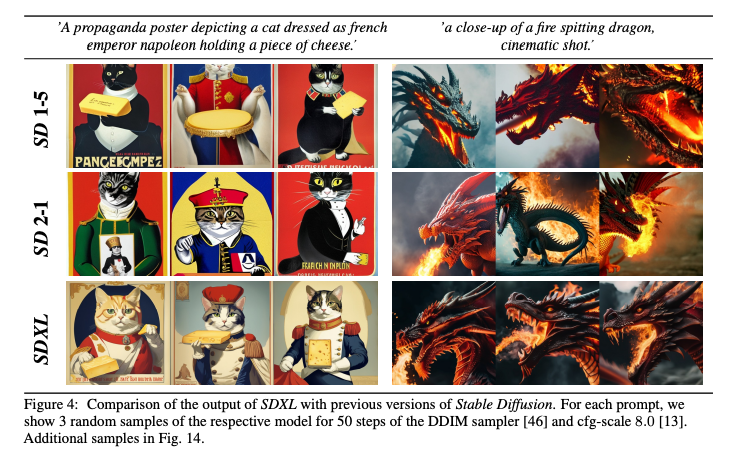
\includegraphics[scale=0.2]{images/crop_example_sdxl}
               \label{fig:crop_example_sdxl}
           \end{figure}~\cite{podell2023sdxl}
        \end{column}
    \end{columns}
\end{frame}



\begin{frame}{Image Refinement}
    \begin{columns}
        \begin{column}{0.4\textwidth}
            \fontsize{7pt}{7pt}\selectfont
            \begin{itemize}
                \item Problem: noisy patches in images
                \item Solution
                \begin{itemize}
                    \item Train model $SD_{edit}$ only on super high-resolution images.
                    \item Diffuse the latent representation of the generated image with noisy patches $z_t$.
                    \item Denoise the diffused $z_t$ with $SD_{edit}$ using same prompt used to generate the image.
                    \item $SD_{edit}$ specialized on the first 200 discrete noise scales.
                \end{itemize}
            \end{itemize}
        \end{column}
        \begin{column}{0.6\textwidth}
           \begin{figure}
               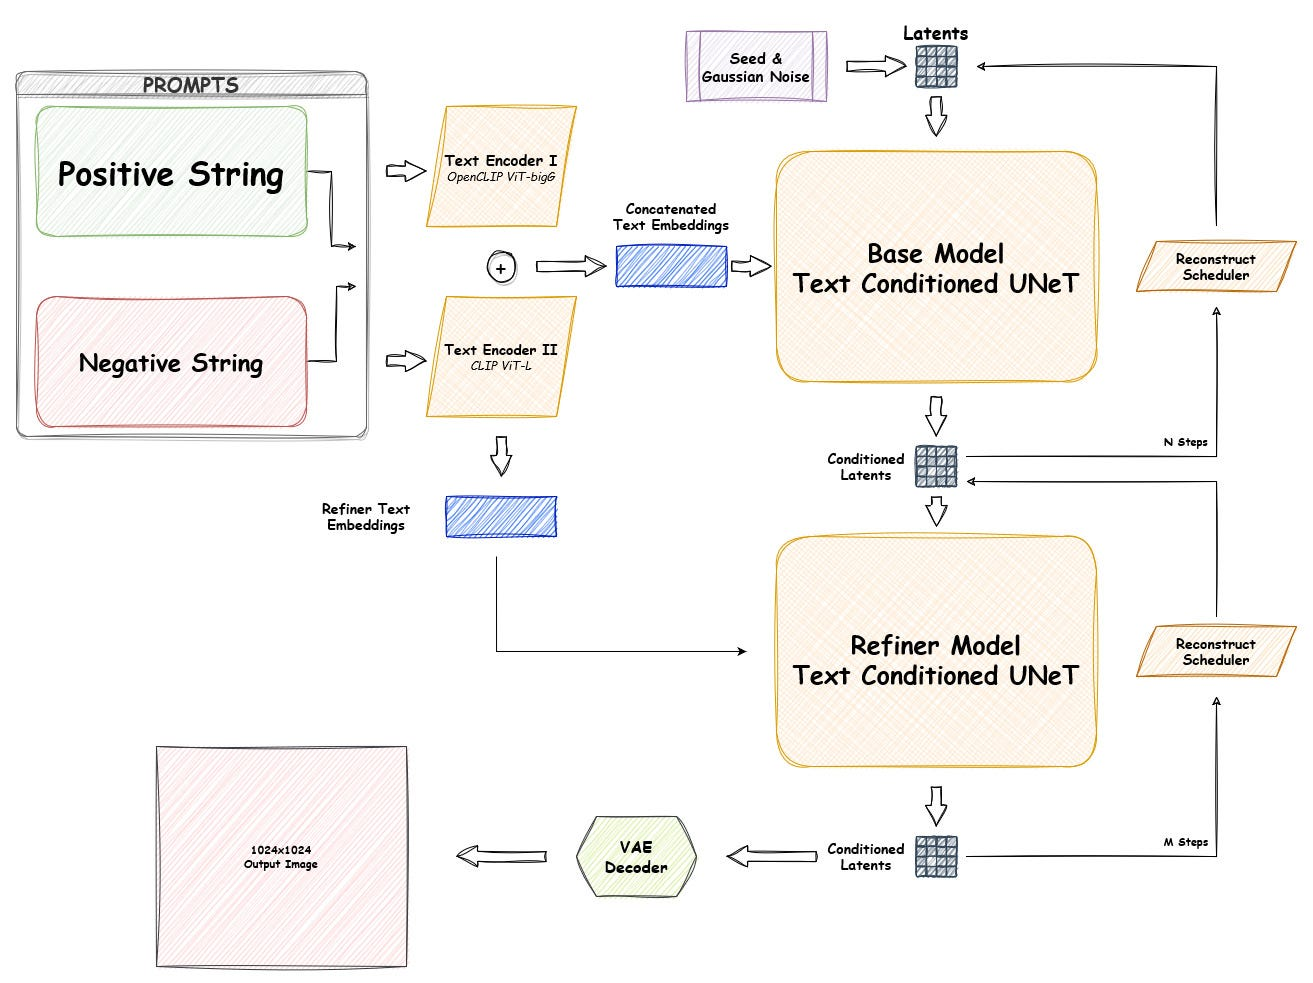
\includegraphics[scale=0.13]{images/sdxl_architecture}
               \label{fig:sdxl_architecture}
           \end{figure}~\cite{demir}
        \end{column}
    \end{columns}
\end{frame}



\begin{frame}{ControlNet}
    ControlNet modifies the SD architecture to allow for conditioning on additional input images.
   \begin{figure}
       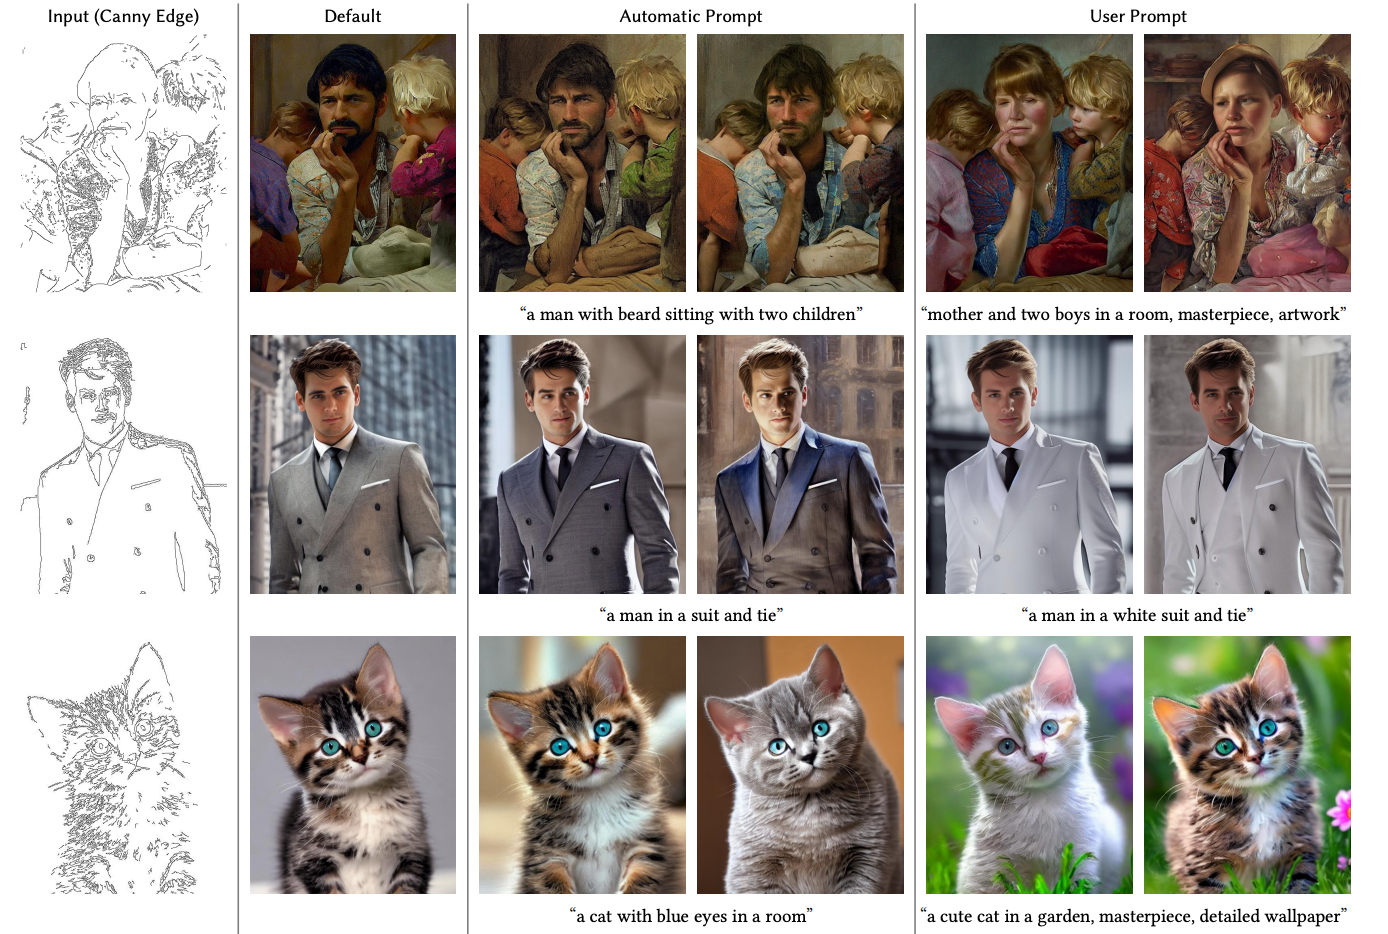
\includegraphics[scale=0.17]{images/control_net_generated_images}
       \label{fig:control_net_generated_images}
   \end{figure}~\cite{zhang2023adding}
\end{frame}



\begin{frame}{ControlNet}
    \begin{columns}
        % left column
        \begin{column}{0.5\textwidth}
            \begin{itemize}
               \item Freezes U-net encoder weights.
               \item Create a \textbf{trainable copy} of the U-net encoder weights.
               \item Conditional input image transformed with simple convolution.
               \item Outputs passed to skip connections of U-nets decoder through a zero-convolution
            \end{itemize}
        \end{column}

        % right column
        \begin{column}{0.5\textwidth}
            \begin{figure}
                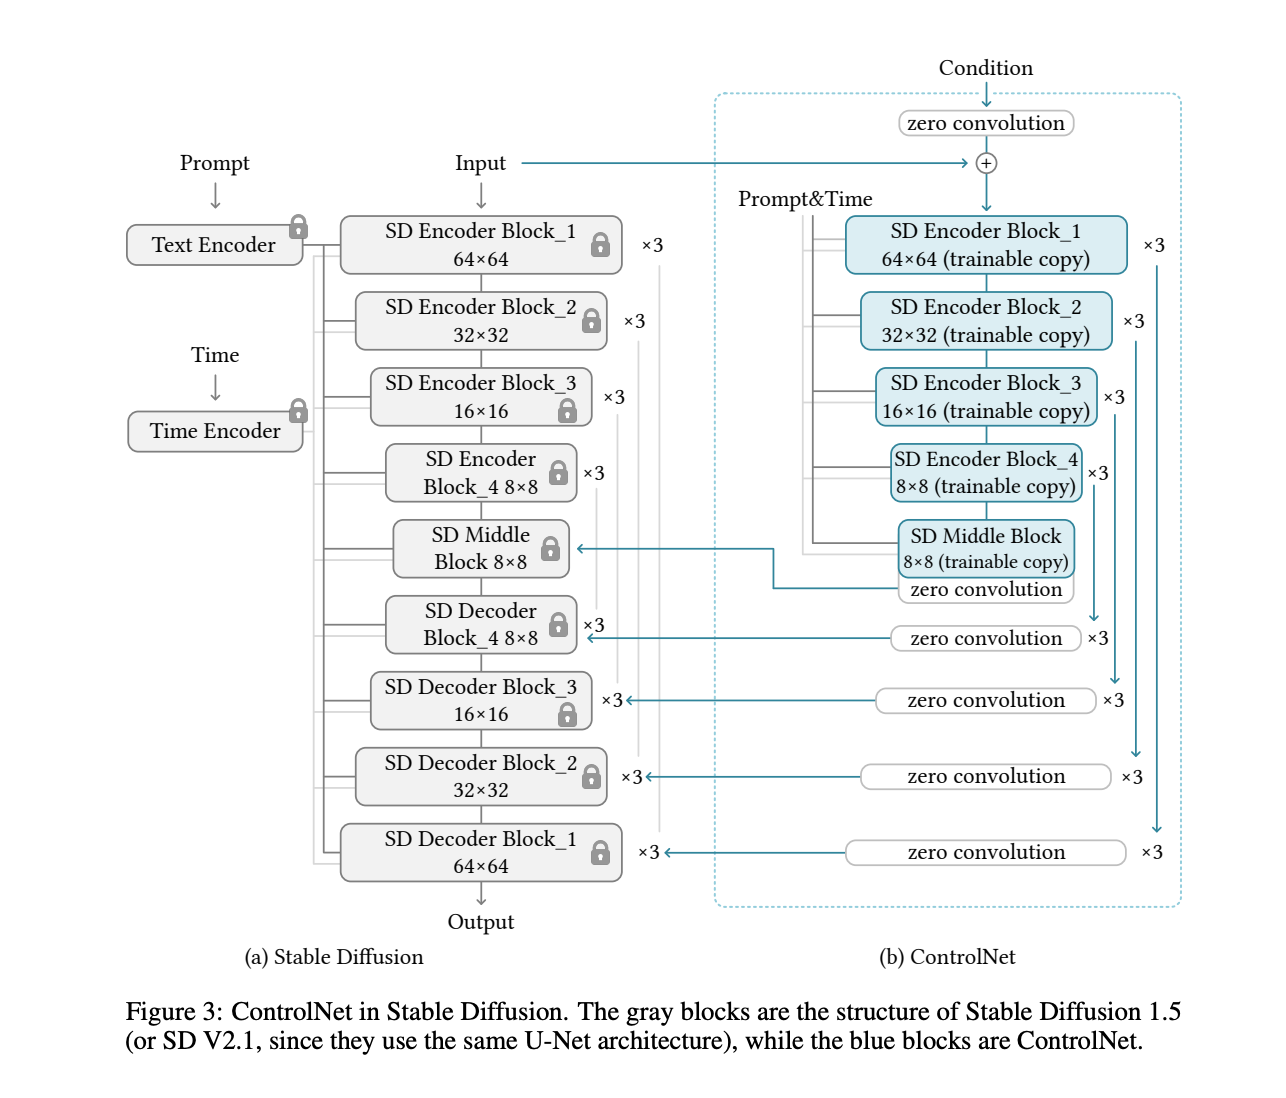
\includegraphics[scale=0.23]{images/control_net_model_architecture}
                \label{fig:control_net_generated_images}
            \end{figure}
        \end{column}
    \end{columns}
\end{frame}



\begin{frame}{Training Flow}
    \begin{itemize}
        \item Choose one conditional input image type (ie canny-edge)
        \item Use a preprocessor to transform your training images into canny-edge versions of the image.
        \item Input is prompt (50\% no prompt), noisy image, and canny-edge image.
        \item Sudden convergence phenomenon: a pre-trained latent diffusion model "abruptly succeeds in following the input conidtioning image; usually in less than 10k optimization steps."~\cite{zhang2023adding}
    \end{itemize}
    \begin{figure}
        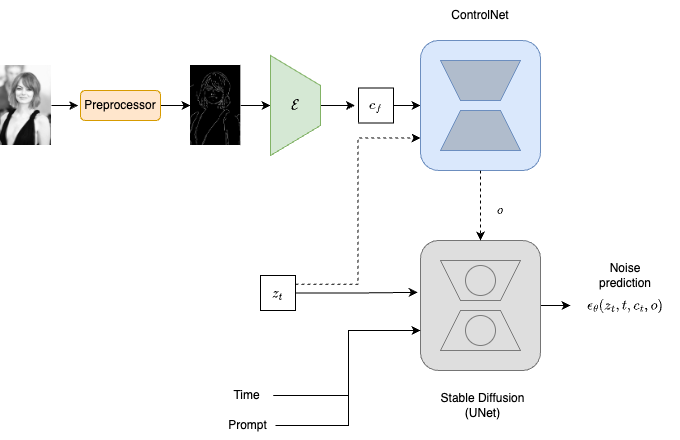
\includegraphics[scale=0.23]{images/cn_training}
        \label{fig:control_net_training}
    \end{figure}
\end{frame}



\begin{frame}{ControlNet training \& objective}
    \fontsize{7pt}{7pt}\selectfont
            \begin{align*}
                l_{ldm} = \mathbb{e}_{z_0, t, c_t, c_f, \epsilon \sim \mathcal{n}(0,1)} \lvert \epsilon - \epsilon_{\theta}(z_t, t, c_t, c_f) \rvert_2^2
            \end{align*}
            \begin{itemize}
                \item $z_0$ input image.
                \item $t$ time step embedding.
                \item $c_t$ text conditioning embedding with 50\% of strings replaced with blanks to place embphasis on control image.
                \item $c_f$ control image embedding.
            \end{itemize}
            \begin{figure}
                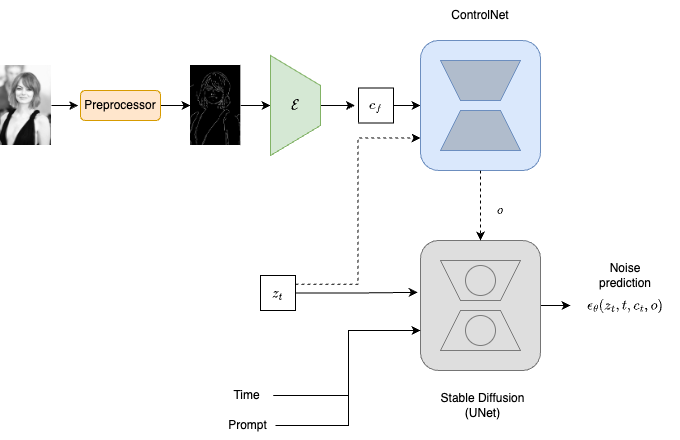
\includegraphics[scale=0.23]{images/cn_training}
                \label{fig:control_net_training}
            \end{figure}
\end{frame}



\begin{frame}{Training}
    \fontsize{7pt}{7pt}\selectfont
    \begin{itemize}
        \item During training, 50\% of text prompts are replaced with empty strings at random, placing emphasis on the conditional image.
        \item One ControlNet model trained per conditional input image type (canny edge, hough line, etc)
    \end{itemize}
    \begin{figure}
        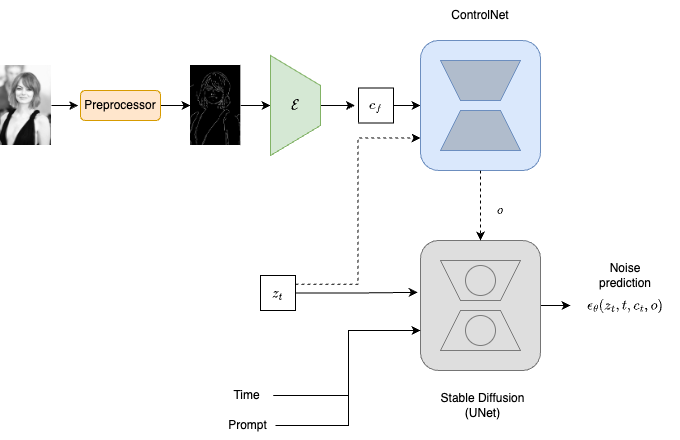
\includegraphics[scale=0.25]{images/cn_training}
        \label{fig:control_net_training}
    \end{figure}
\end{frame}



\begin{frame}{Prompt}
    \fontsize{7pt}{7pt}\selectfont
    Controlnet performs well without prompt guidance.
    \begin{figure}
        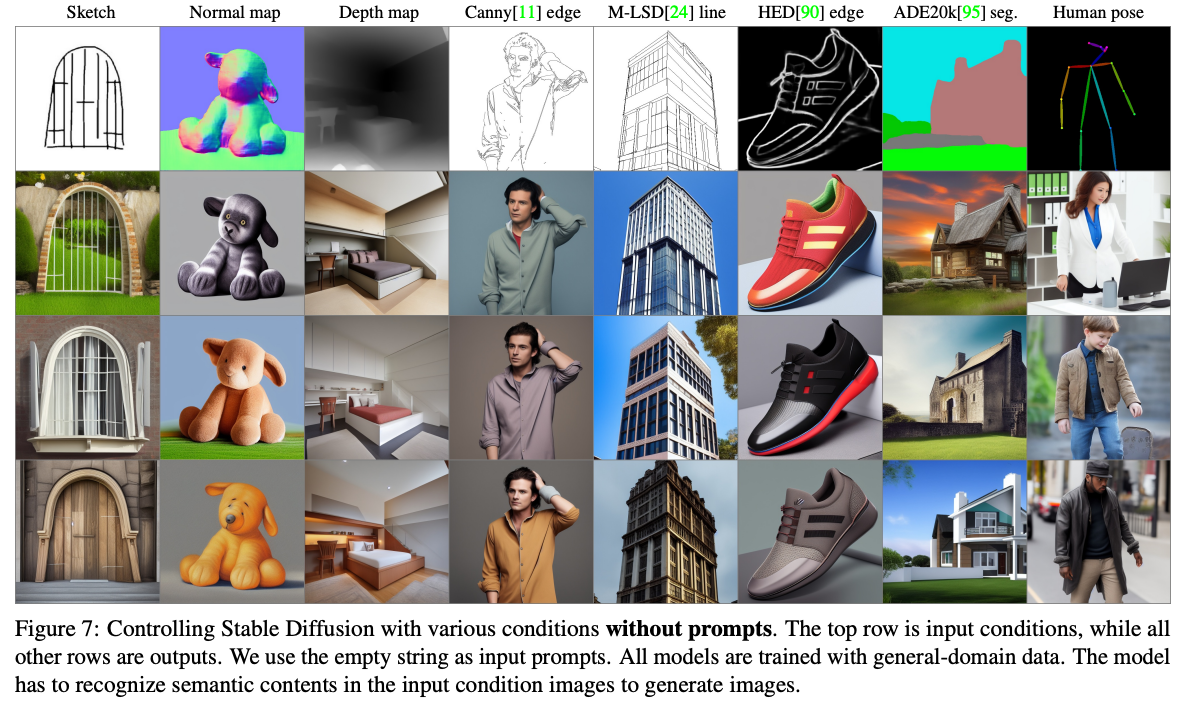
\includegraphics[scale=0.2]{images/cn_no_prompt}
        \label{fig:control_net_training}
    \end{figure}
\end{frame}



\begin{frame}{Ablative Study}
    \fontsize{7pt}{7pt}\selectfont
    The conditional input image is powerful.
    \begin{figure}
        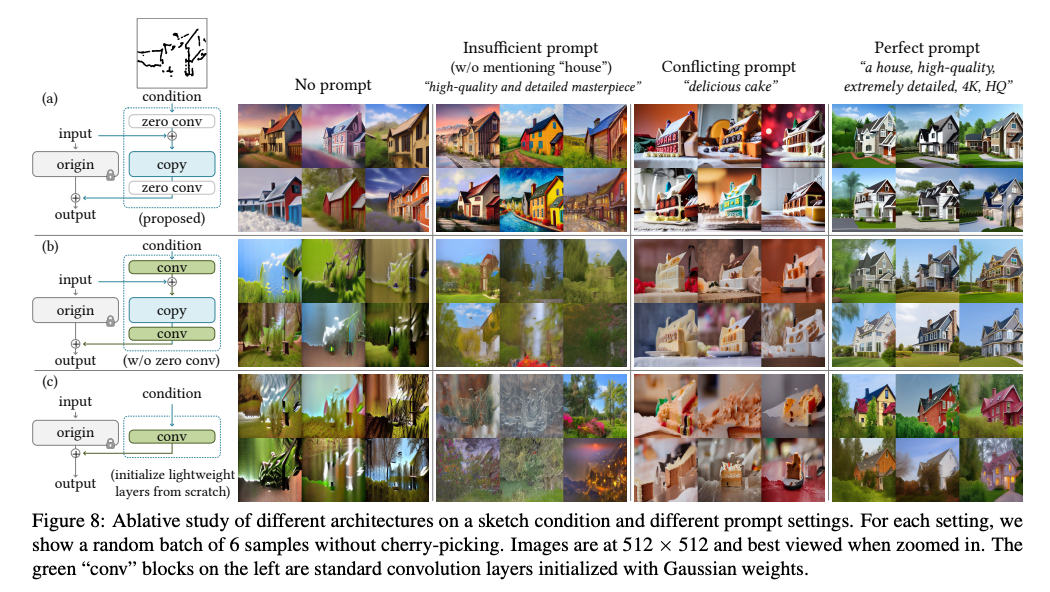
\includegraphics[scale=0.2]{images/cn_input_variation}
        \label{fig:control_net_training}
    \end{figure}
\end{frame}



\begin{frame}{Composability}
    \fontsize{7pt}{7pt}\selectfont
    Controlnet is composable. do we train several ControlNets on one SD model?
    \begin{figure}
        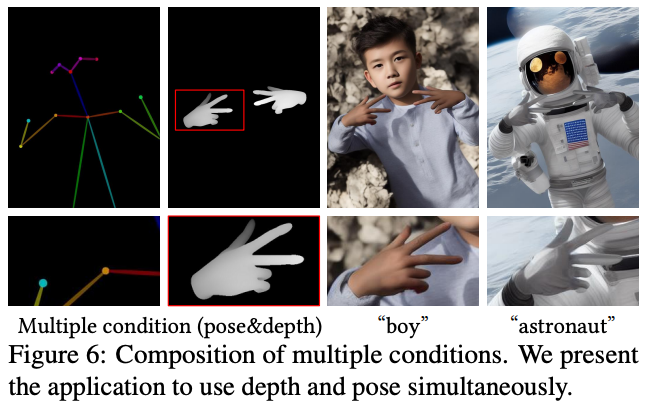
\includegraphics[scale=0.2]{images/cn_composition}
        \label{fig:control_net_training}
    \end{figure}
\end{frame}



\begin{frame}{Classifier-free guidance resolution weighting}
    CFG resolution weighting for controlnet
    \begin{itemize}
        \item If left unmodfied, controlnet will add the conditional image to both $\epsilon_{uc}$ and $\epsilon_c$.
        \item The conditional guidance on $\epsilon_{uc}$ will nullify the masked prompt, removing cfg.
        \item If added only to $\epsilon_c$, the model will place to much emphasis on the conditional image.
    \end{itemize}
\end{frame}



\begin{frame}{Classifier-free guidance resolution weighting}
    \fontsize{7pt}{7pt}\selectfont
    \begin{columns}
        \begin{column}{.5\textwidth}
            Solution: Leverage the scaling properties inherent to the architecture to weight CFG.
            \begin{itemize}
                \item Add the conditional image to $\epsilon_c$
                \item Mulitply each connection between stable diffusion and controlnet by a weight that reduces the strength of the conditional image according to the resolution of each block
            \end{itemize}
        \end{column}
        \begin{column}{.5\textwidth}
            \begin{figure}
                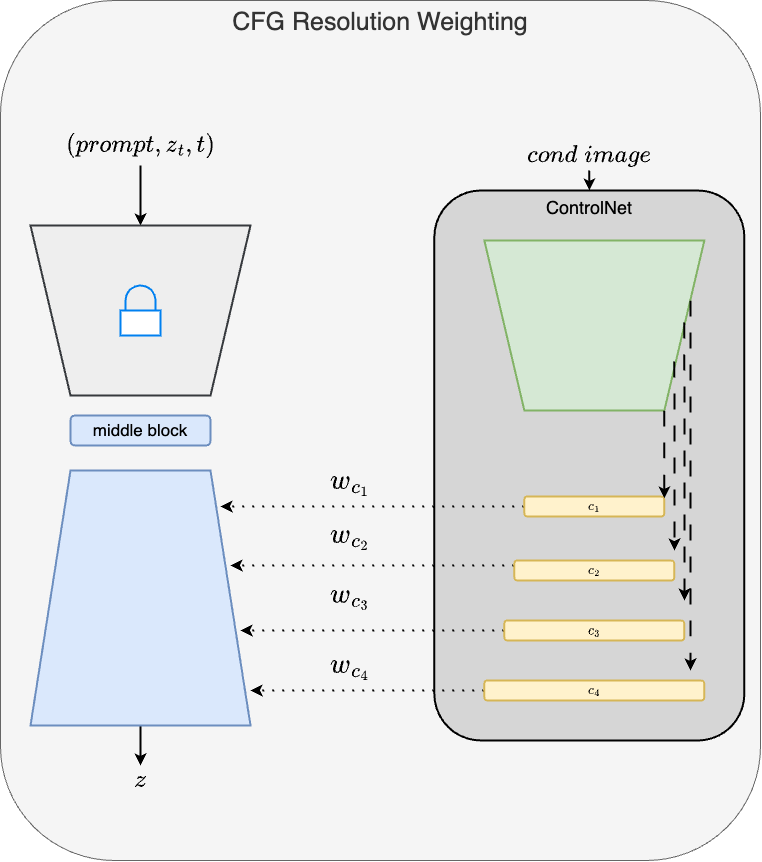
\includegraphics[scale=0.2]{images/cfg_resolution_weighting}
                \label{fig:cfg_resolution_weighting}
            \end{figure}
        \end{column}
    \end{columns}
\end{frame}



\section{\bibname}
\begin{frame}[t, allowframebreaks]{\bibname}
    \printbibliography[heading=none]
\end{frame}

\end{document}
